\documentclass[10pt,a4paper]{article}
\usepackage[utf8]{inputenc}
\usepackage[scale=0.7,vmarginratio={1:2},heightrounded]{geometry}

\usepackage[numbers]{natbib}

% link support in pdf
\usepackage[colorlinks,allcolors=blue,breaklinks = true]{hyperref}

% images in pdf
\usepackage{graphicx}
\graphicspath{{Bilder/}}
% multiple images
\usepackage{subfigure}
% images float in text
\usepackage{float}

% url support
\usepackage{url}
% glossarie support
\usepackage[acronym, automake]{glossaries}
\makeglossaries
\loadglsentries{glossary}

% math libs
\usepackage{amsmath}
\usepackage{amssymb}
\usepackage{amstext}
\usepackage{amsfonts}
\usepackage{mathrsfs}

% Code formating
\usepackage{listings}
\usepackage{color}

\definecolor{dkgreen}{rgb}{0,0.6,0}
\definecolor{gray}{rgb}{0.5,0.5,0.5}
\definecolor{mauve}{rgb}{0.58,0,0.82}

\lstset{frame=tb,
  language=Java,
  aboveskip=3mm,
  belowskip=3mm,
  showstringspaces=false,
  columns=flexible,
  basicstyle={\small\ttfamily},
  numbers=none,
  numberstyle=\tiny\color{gray},
  keywordstyle=\color{blue},
  commentstyle=\color{dkgreen},
  stringstyle=\color{mauve},
  breaklines=true,
  breakatwhitespace=true,
  tabsize=3
}

%Metadata
\title{TBD}
\author{Simon Hischier}
\date{April 2018}

\begin{document}

%Titlepage
\begin{titlepage}
%\maketitle
\centering
\vspace{1cm}
	{\scshape\LARGE Fachhochschule Luzern HSLU \par}
	\vspace{1cm}
	{\scshape\Large Studiengang Digital Ideation, Bachelor \par}
	
	{\scshape\Large 4. Semester\par}
	\vspace{1.5cm}
	{\huge\bf Procedural Generation in the age of AI\par}
	
	\vspace{10cm}
	{\Large Simon Hischier\par}
	\vfill

% Bottom of the page
	{\large \today\par}
\end{titlepage}

%Table of Contents Page
\renewcommand{\contentsname}{Inhalt}
\tableofcontents
\newpage

%First real page
\section{Abstract}
bliblablup todo

\section{Procedural Generation}
The term \gls{pc} ..

\section{AI, Machinelearning, Deeplearning}
\label{sec:AIMachinelearningDeeplearning}
blibla \cite{MichaelCopeland2016} TODO: research definitions
\begin{figure}[H]§
	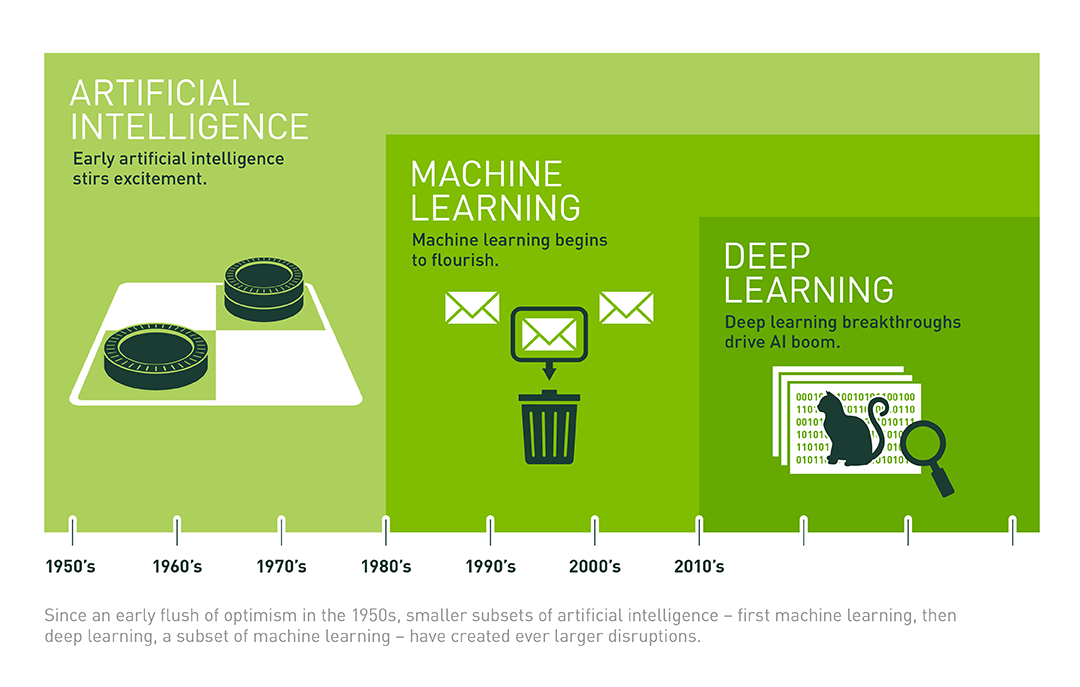
\includegraphics[width=\textwidth, height=\textheight, keepaspectratio]{Deep_Learning_Icons_R5.png}
	\caption{Levels of AI as Image. \cite{MichaelCopeland2016}}
\end{figure}

\section{Motivation}
The early days of PC games were all about \gls{pc} TODO: https://ieeexplore.ieee.org/abstract/document/5593333/
Games that are meant to be replayed a lot benefit from Procedural Generation.

\section{Recurrent Neural Networks}
As explained in \autoref{sec:AIMachinelearningDeeplearning} \gls{ml} is a broad term and includes a variety of models. The \gls{rnn} are networks for tasks where we need some kind of persistance. If we want to classify videoframes the network should have some kind of consistency.\cite{Olah2015} A network should persist the last seen data and not reclassify items every frame. Reclassifying without previous context could lead to different recognitions in every frame for the same object.

\section{Long short-term memory}
\gls{rnn} are good for persisting very recent information. Sentences are a great example: "Ships are built to float on \textit{water}". The \gls{rnn} is great in filling the end of this sentence. Problems arise when the information is needed a lot later. The more information is inbetween the contextual references the more unreiable a basic \gls{rnn} gets. Books for example can have references on the last page to the very beginning. For such tasks a \gls{lstm} model is the perfect fit. The \gls{lstm} network was introduced by Hochreiter Sepp and Urgen Schmidhuber\citep{Hochreiter1997}. A \gls{lstm} is a specialized version of a \gls{rnn} which is designed for these kind of tasks. Almost all \gls{rnn} tasks can be achieved with a \gls{lstm} \gls{rnn} \cite{Olah2015}. 
to read: $https://en.wikipedia.org/wiki/Long_short-term_memory$
$https://colah.github.io/posts/2015-08-Understanding-LSTMs/$



\section{OLD:}
\section{TensorFlow.js}
As of April 2018 Google released a new JavaScript \gls{ml} library called \gls{tensorflowjs}. \gls{tensorflowjs} is build on deeplearn.js and can be used for a broad variety of \gls{ml} tasks. The library allows to train and run models in the webbrowser. Models can be pre-trained on a server or offline computer and then be used on the website.

\section{Challenges}
various challenges:
\begin{itemize}
\item level is playable
\item Levels getting harder
\item build up, learn new thing and then master it
\end{itemize}


\section{Goal}
The goal of this work is to generate maps for games. Maps from "Super Mario" or "Super Meat Boy" contain mostly solid or empty blocks. With that knowledge, the levels can probably be represented in an easy to read text format instead of an image format. The text can probably be feed into an \gls{ml} system and new maps can be generated with the assistance of a \gls{ml} model.

\section{examples}

We can Cite \cite{wikipediaScriptingLanguage}, \cite{Iivari2008usabilityInCompanyOSS}, \cite{almarzouq2005open}, \cite{heiseonline2017limuxservus}, \cite{viorres2007major}, \cite{wikipediaScriptingLanguage} etc. If we want to have terms and shortcuts we can introduce them once: \gls{longGlsEx} and \gls{oss}. If we refer to \gls{longGlsEx} and \gls{oss} later it will only use the short version.

\newpage
\newpage

\section{Examples}
\section{Examples of Images}
Images are possible aswell:
\begin{figure}[H]
	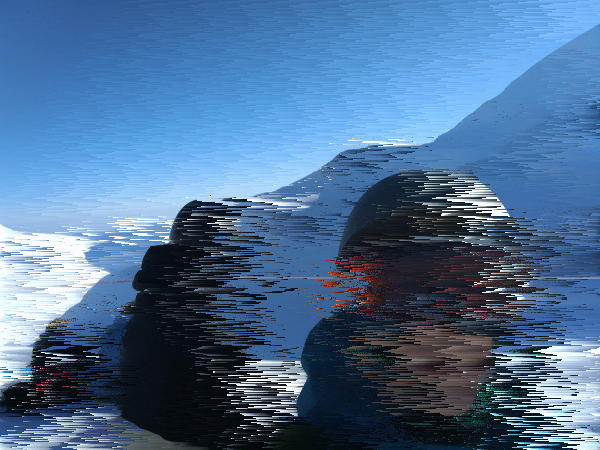
\includegraphics[width=\textwidth, height=\textheight, keepaspectratio]{example1.png}
	\caption{Thats me. Source: {https://thecell.eu/}}
\end{figure}

and even multiple images are possible

\begin{figure}[H]
	\centering
	\subfigure{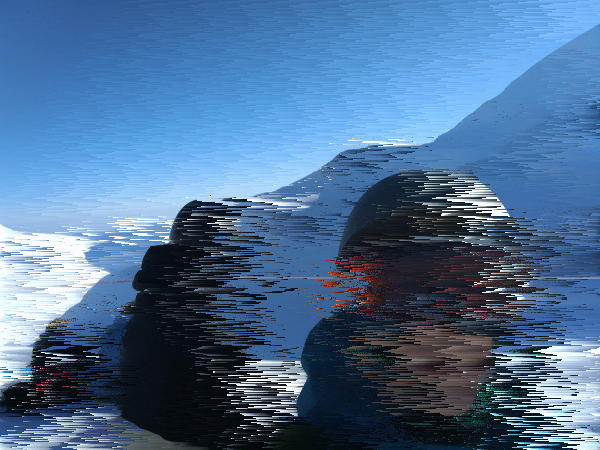
\includegraphics[width=0.4\textwidth]{example1.png}}
	\subfigure{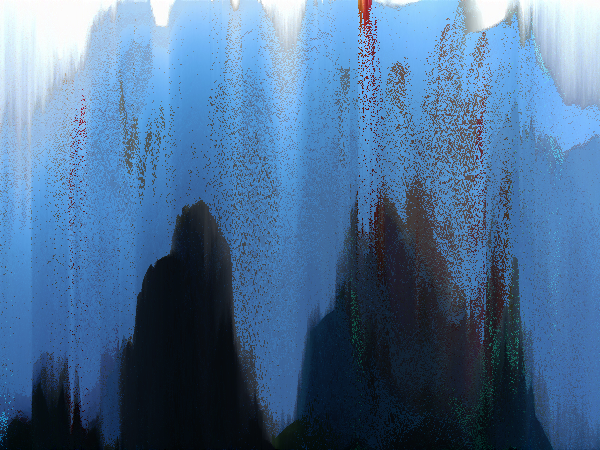
\includegraphics[width=0.4\textwidth]{example2.png}}
	\subfigure{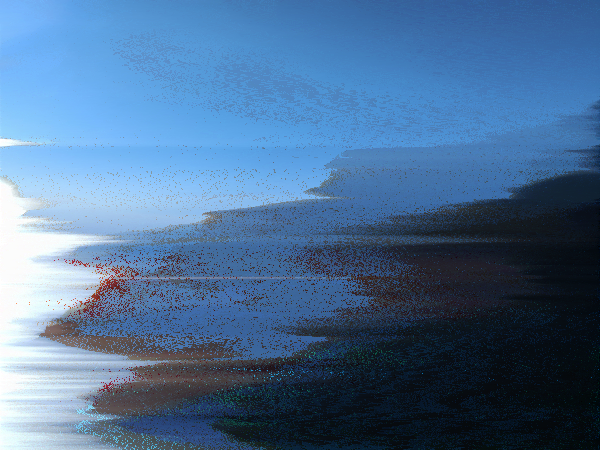
\includegraphics[width=1\textwidth]{example3.png}}
	\caption{multiple images as an example}
	\caption{if needed to reference separate it's possible like this}
\end{figure}

\section{Script code}
A simple codeblock is possible take a look at this:
\begin{lstlisting}
<script>
let aVar = "this is a JavaScript variable";
console.log(aVar);
</script>
\end{lstlisting}

\section{Tables etc.}

\textbf{Lists} can be made as following:
\begin{itemize}
\item List an item once
\item or twice
\item just add more if needed
\item sublists are possible aswell:
\begin{itemize}
\item List an item once
\item or twice
\item just add more if needed
\end{itemize}
\end{itemize}

If you are looking for tables, here it is:
\begin{table}[H]
\centering
\begin{tabular}{ |c|c|c|c|c|c|c| }
\hline
 & 1 & 2 & 3 & 4 & 5 & 6 \\
\hline
Dota 2 & 31 min & H & ++ & Z & $<$40\$ & Kosmetisch \\
\hline
PoE & $\infty$ & H & ++ & Z & $<$\$440 & Shoppunkte \\
\hline
The Witcher 3 & 48.5h & H \& C &  & Z & \$24 & AddOn \\
\hline
\end{tabular}
\caption{Statistik Spiellänge wurde erfasst von \texttt{https://howlongtobeat.com} und \texttt{http://steamspy.com/.}}
\label{table:1}
\end{table}

\section{Referenzen und Akronyme}

\printglossaries

%\renewcommand{\refname}{myBibliography}
\bibliography{myBibliography}
%\bibliographystyle{unsrtnat}
%\bibliographystyle{plainnat}
\bibliographystyle{unsrt}
%\bibliography{myBibliography}

%list the figures and tables in contents
%\addcontentsline{toc}{section}{\listfigurename}
%\addcontentsline{toc}{section}{\listtablename}

%print list
\listoffigures
\listoftables

%\nocite{*}

\end{document}